This Section describes the architectures of the legacy, based on Hudi the system implemented during this thesis work, based on Iceberg, and the system implemented in a related thesis work \cite{manfrediReducingReadWrite2024}, based on Delta Lake. Those are the system that will be run and measured in teh experimental part of this thesis work. This Section is divided into six Subsections, according to the system and the operation run over it. For each Subsection, a chart presents the operation protocol step by step.



%%%% HUDI WRITE
\subsection{Legacy system - Hudi - writing}
\label{subsec:back_sys_hudi_write}

Figure \ref{fig:hudi_write}~\footnote{For enhanced visualization, refer Figure.} shows the legacy Hopsworks feature store write process from the client onto the offline feature store.  \todo{Add reference to appendix}The process is mainly split into two synchronous parts: upload and materialization. In the upload step, the Pandas DataFrame given as input is converted into rows and sent to Kafka one row at a time. Then, when the upload is completed, the client will be notified. Asynchronously, a Spark job, the Hudi Delta Streamer, has been running in the cluster since the Hopsworks cluster was started. This job periodically retrieves messages from Kafka, and then once it retrieves a full table, it writes the table in a column-oriented format to Apache Hudi, which sits on top of a \gls{HopsFS} system. Once the materialization is completed, the Python client will be notified of completion.

As in the pipeline, the upload and the materialization are two parts of the process that do not act synchronously. During the experimental part of the thesis, the materialize function was called to measure the latency of the whole process without having to account for the Hudi Delta Streamer data retrieval period. This allows the system to perform the materialization on call instead of waiting for the period. This enabled the experiments to retrieve accurate data on the total latency of the process.

\begin{figure}
    \begin{center}
      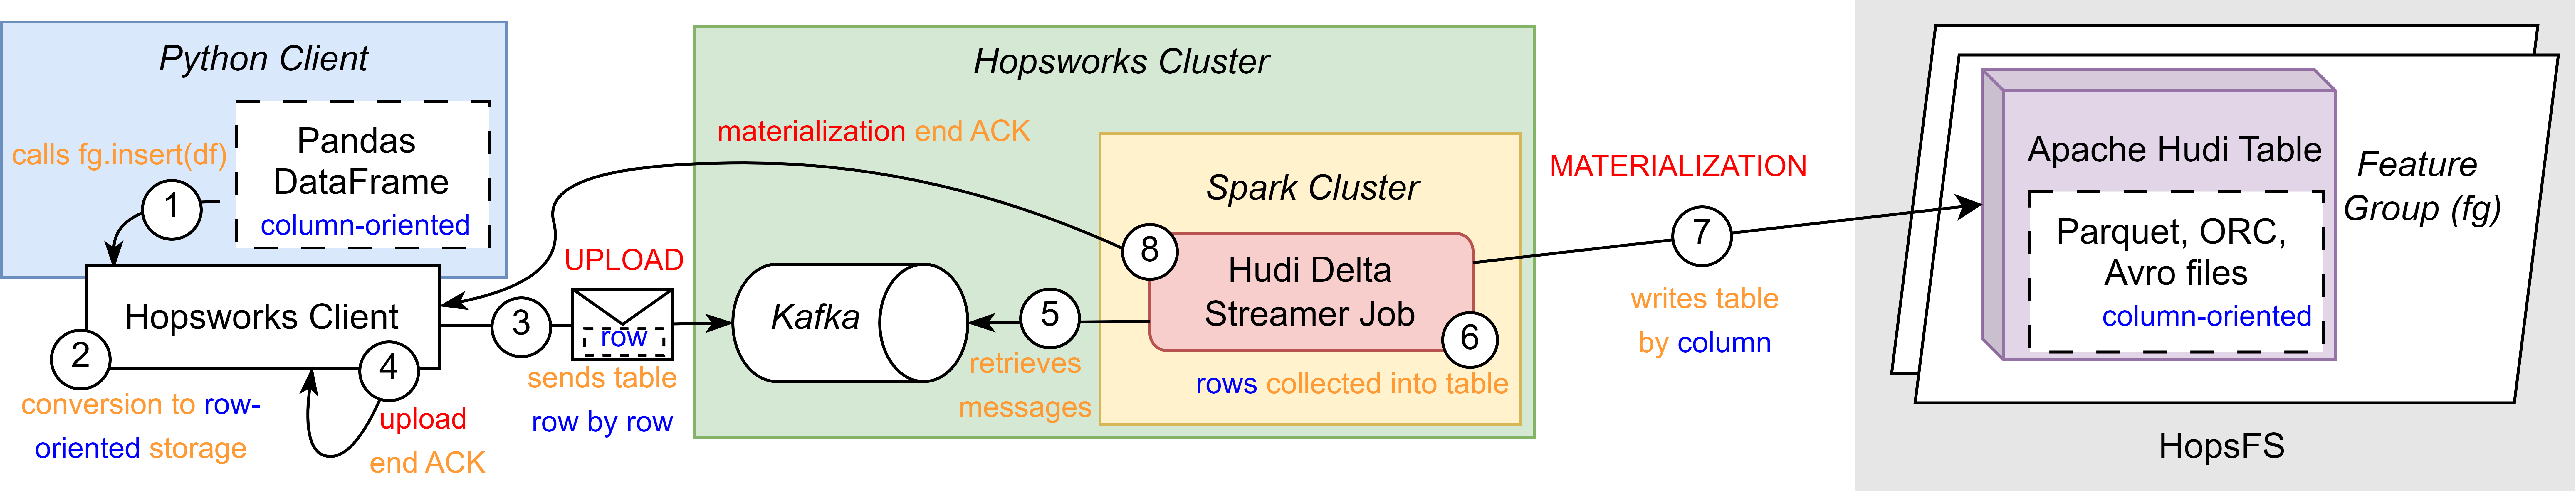
\includegraphics[width=\textwidth]{figures/2-background_and_related_work/hudi_write.png}
    \end{center}
    \caption[Legacy system - Hudi - write process]{Legacy system writing a Pandas DataFrame from a Python client to the Hopsworks offline feature store. Each step is represented with a number. The table format conversion is outlined in blue, i.e., from columns to rows and then from row to columns. Steps from one to four represent the upload process, while the materialization process is complete at step eight. The diagram was realized based on one-to-one interviews with Hopsworks AB employees developing the Hopsworks feature store.}
    \label{fig:hudi_write}
\end{figure}



%%%% HUDI READ
\subsection{Legacy system - Hudi - reading}
\label{subsec:back_sys_hudi_read}

Figure \ref{fig:hudi_read}~\footnote{For enhanced visualization, refer Figure.}  \todo{Add reference to appendix}shows the offline feature store. Unlike the writing process, the process is not Spark-based and uses a Spark alternative: a combination of an Arrow Flight server and a DuckDB instance. This avoids the conversion into row-based tables for sending the data, keeping the unified standard Arrow Table, which is a column-oriented format.

\begin{figure}
    \begin{center}
      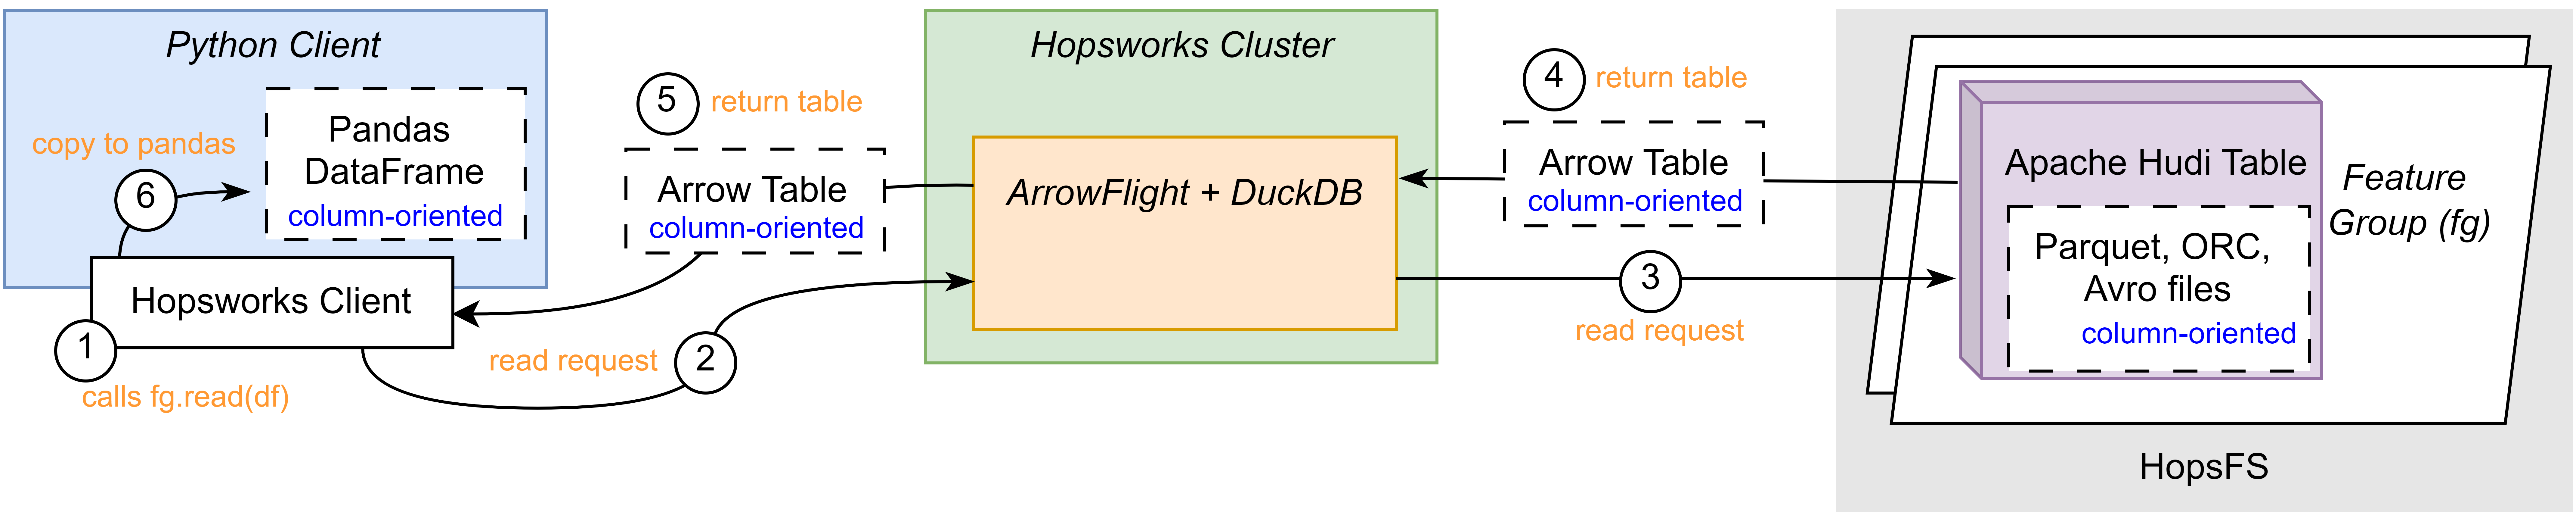
\includegraphics[width=\textwidth]{figures/2-background_and_related_work/hudi_read.png}
    \end{center}
    \caption[Legacy system - read process]{Legacy system reading a table from the Hopsworks offline feature store and loading it into the Python client's local memory. The process is streamlined using Arrow Tables that avoid table conversion. Diagram inspired by the Hopsworks feature store paper \cite{10.1145/3626246.3653389}.}
    \label{fig:hudi_read}
\end{figure}



%%%%% ICEBERG WRITE
\subsection{New system - Iceberg - writing}
\label{subsec:back_sys_iceberg_write}

Figure \ref{fig:iceberg_write} shows how the PyIceberg library writes on an Iceberg table instanced on top of \gls{HopsFS}. If first requests metadata information about the existing table to Iceberg Catalog, implemented using SQLite in the example. Once the JSON file containing the metadata is received, it reads the table location and request to read the table. The PyIceberg library streamlines the process without passing from a server instance (Spark), removing the middle-tier from the process.

\begin{figure}
    \begin{center}
      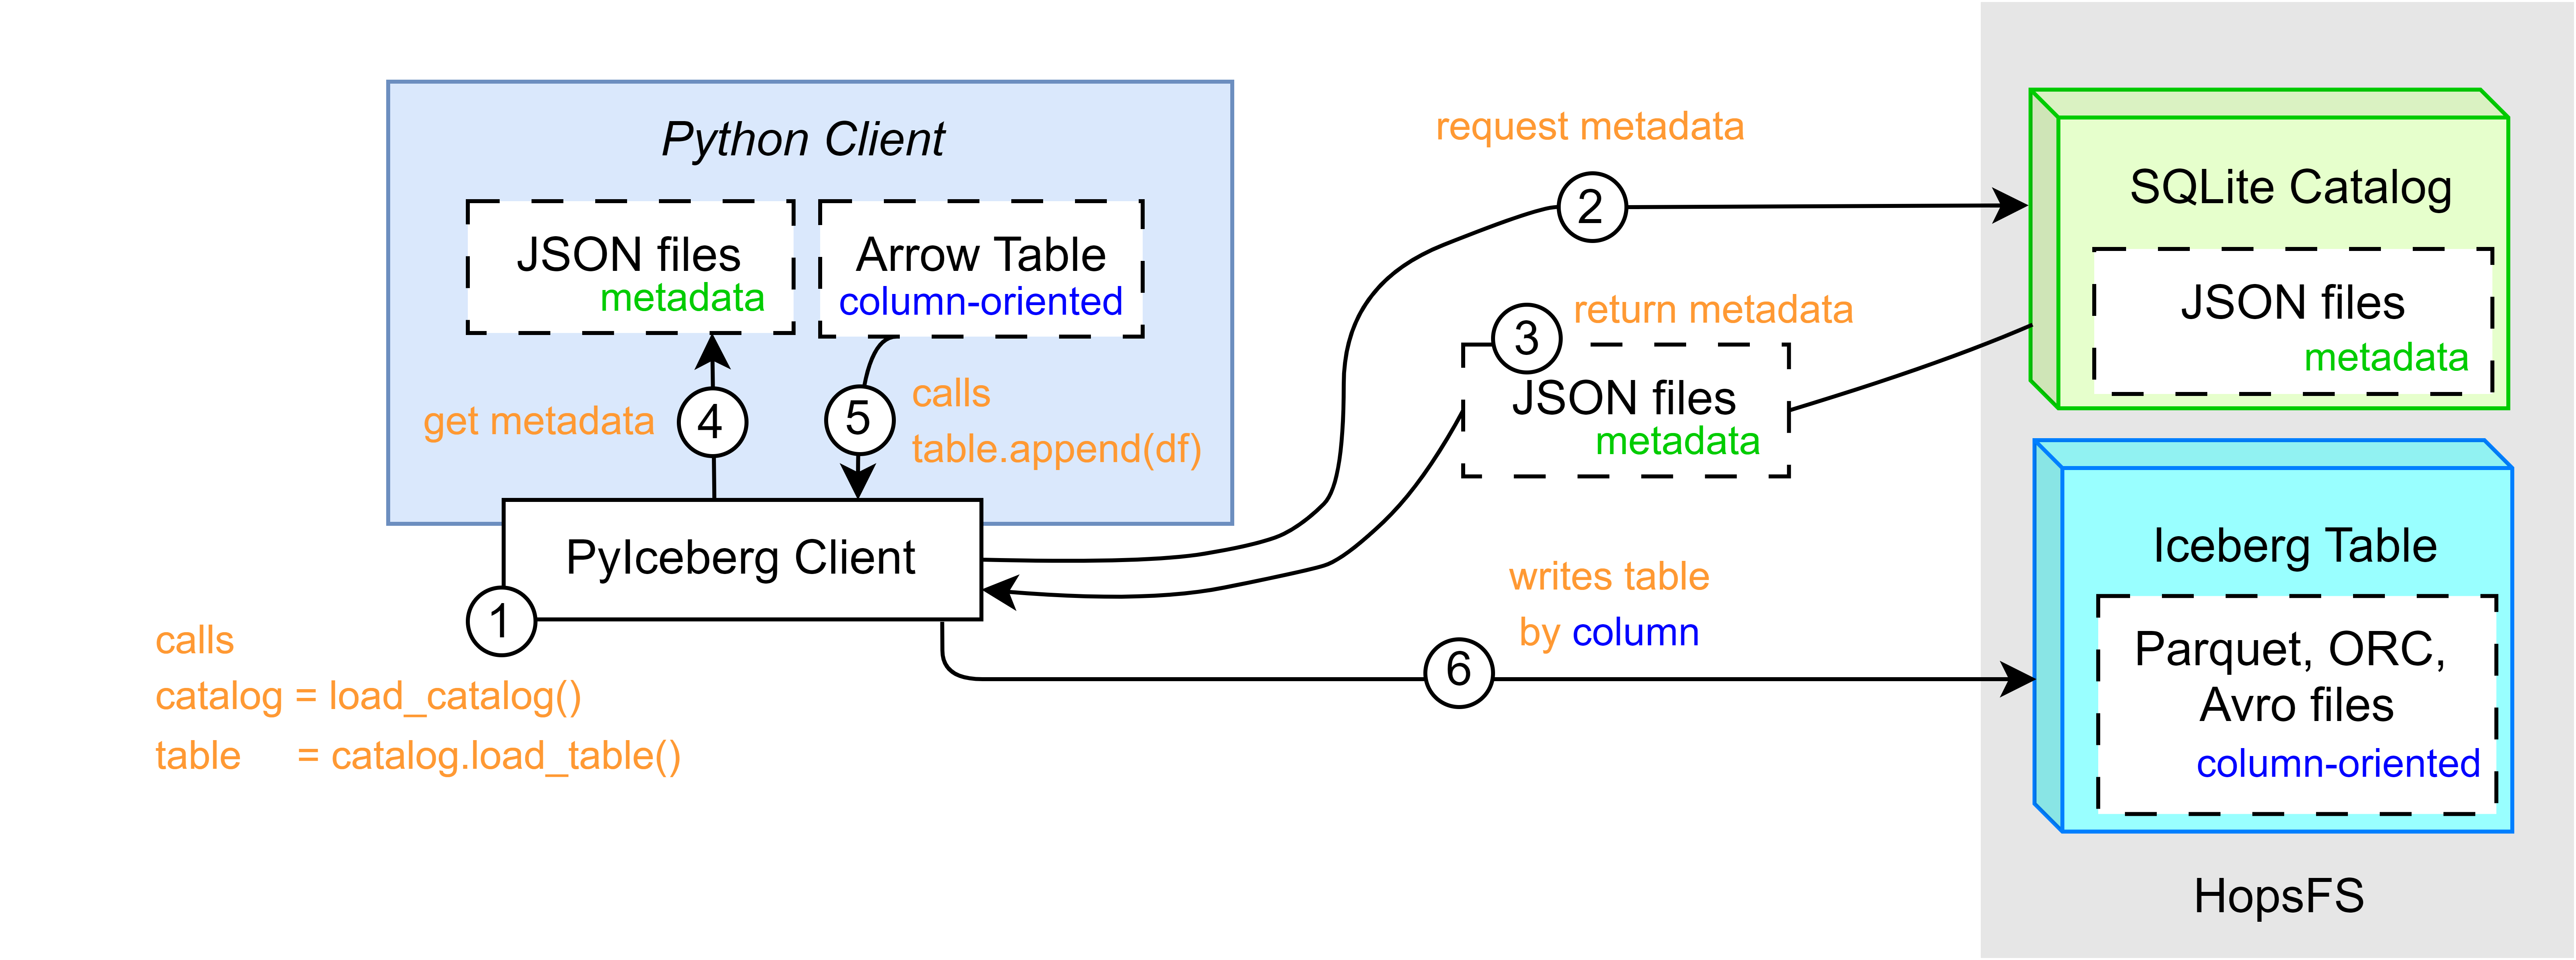
\includegraphics[width=\textwidth]{figures/2-background_and_related_work/iceberg_write.png}
    \end{center}
    \caption[New system - Iceberg - write process]{PyIceberg library writing an Arrow Table from a Python client to an Iceberg Table stored on \gls{HopsFS}.}
    \label{fig:iceberg_write}
\end{figure}



%%%%% ICEBERG READ
\subsection{New system - Iceberg - reading}
\label{subsec:back_sys_iceberg_read}

Figure \ref{fig:iceberg_read} shows how the PyIceberg library reads on an Iceberg table instanced on top of \gls{HopsFS}. If first requests metadata information about the existing table to Iceberg Catalog, implemented using SQLite in the example. Once the JSON file containing the metadata is received, it reads the table location and proceed to write (append), by column, on the Iceberg Table. The PyIceberg library streamlines the process without passing from a server instance (Arrow Flight), removing the middle-tier from the process.

\begin{figure}
    \begin{center}
      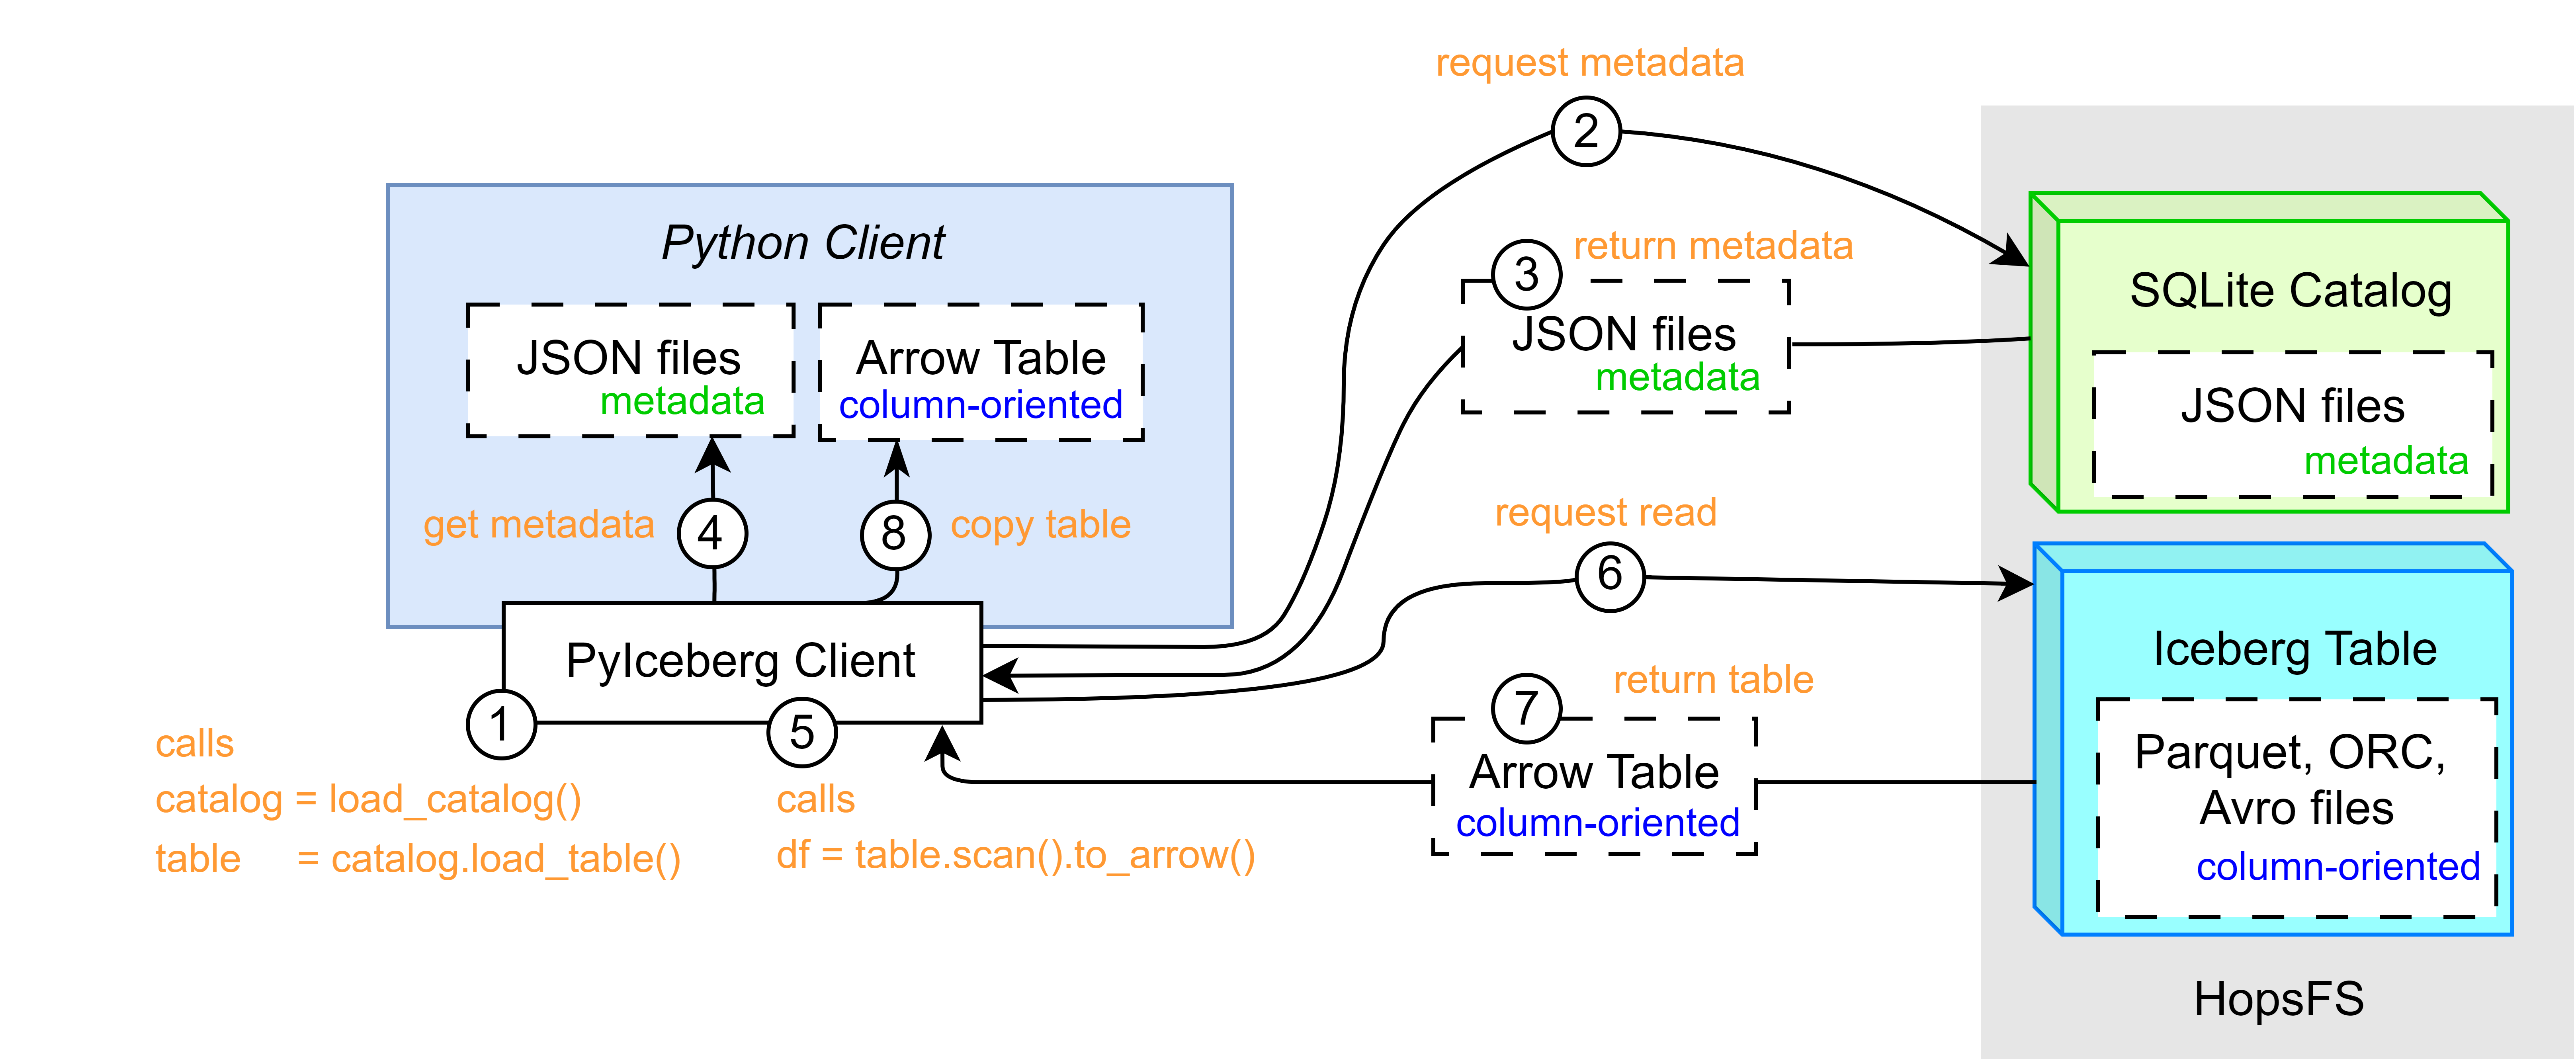
\includegraphics[width=\textwidth]{figures/2-background_and_related_work/iceberg_read.png}
    \end{center}
    \caption[New system - Iceberg - read process]{PyIceberg library reading an Iceberg Table stored on \gls{HopsFS} and loading it into memory.}
    \label{fig:iceberg_read}
\end{figure}



%%%%% DELTA LAKE WRITE
\subsection{New system - Delta Lake - writing}
\label{subsec:back_sys_delta_write}

Figure \ref{fig:delta_write} shows how the delta-rs library writes on a Delta Lake table instanced on top of \gls{HopsFS}. The delta-rs library streamlines the process without passing from a server instance (Spark), removing the middle-tier from the process. In this system, the only file format supported is Parquet, while the other systems supported also ORC and Avro.

\begin{figure}
    \begin{center}
      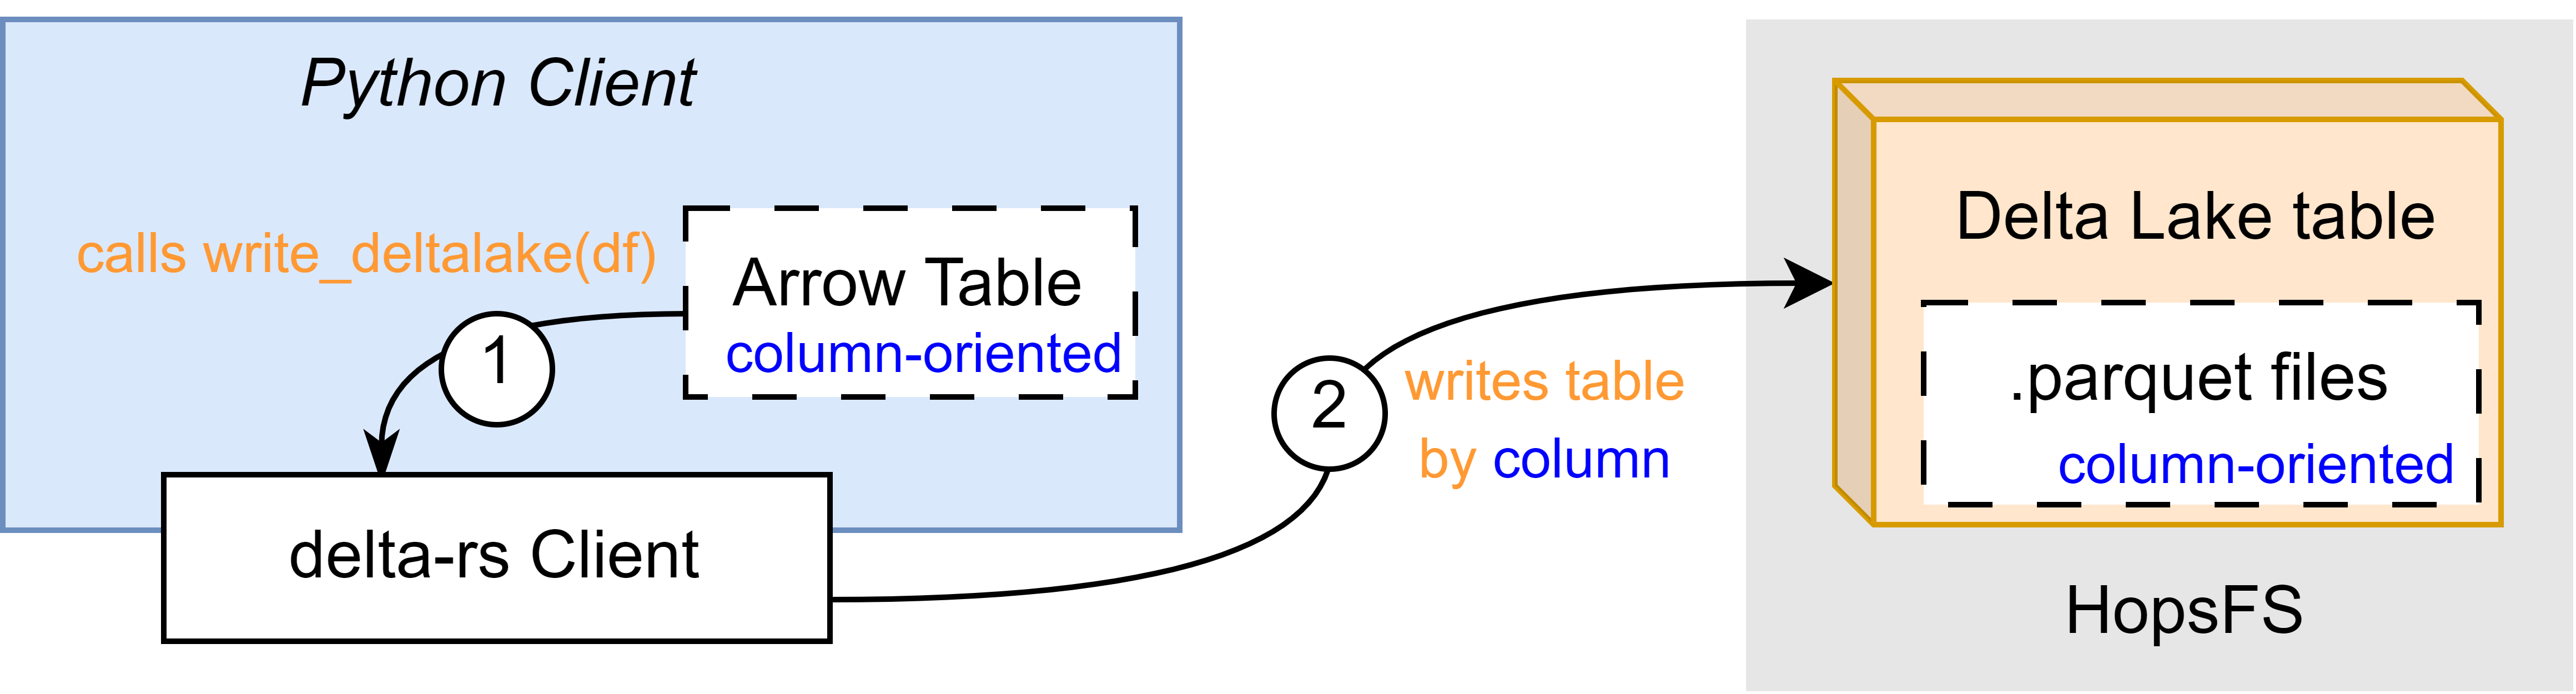
\includegraphics[width=\textwidth]{figures/2-background_and_related_work/delta_write.png}
    \end{center}
    \caption[New system - Delta Lake - write process]{Delta-rs library writing an Arrow Table from a Python client to a Delta Lake table stored on \gls{HopsFS}.}
    \label{fig:delta_write}
\end{figure}



%%%%% DELTA LAKE READ
\subsection{New system - Delta Lake - reading}
\label{subsec:back_sys_delta_read}

Figure \ref{fig:delta_read} shows how the delta-rs library reads a Delta Lake table instanced on top of \gls{HopsFS}. The delta-rs library streamlines the process without passing from a server instance (Arrow Flight), removing the middle-tier from the process. In this system, the only file format supported is Parquet, while the other systems supported also ORC and Avro.

\begin{figure}
    \begin{center}
      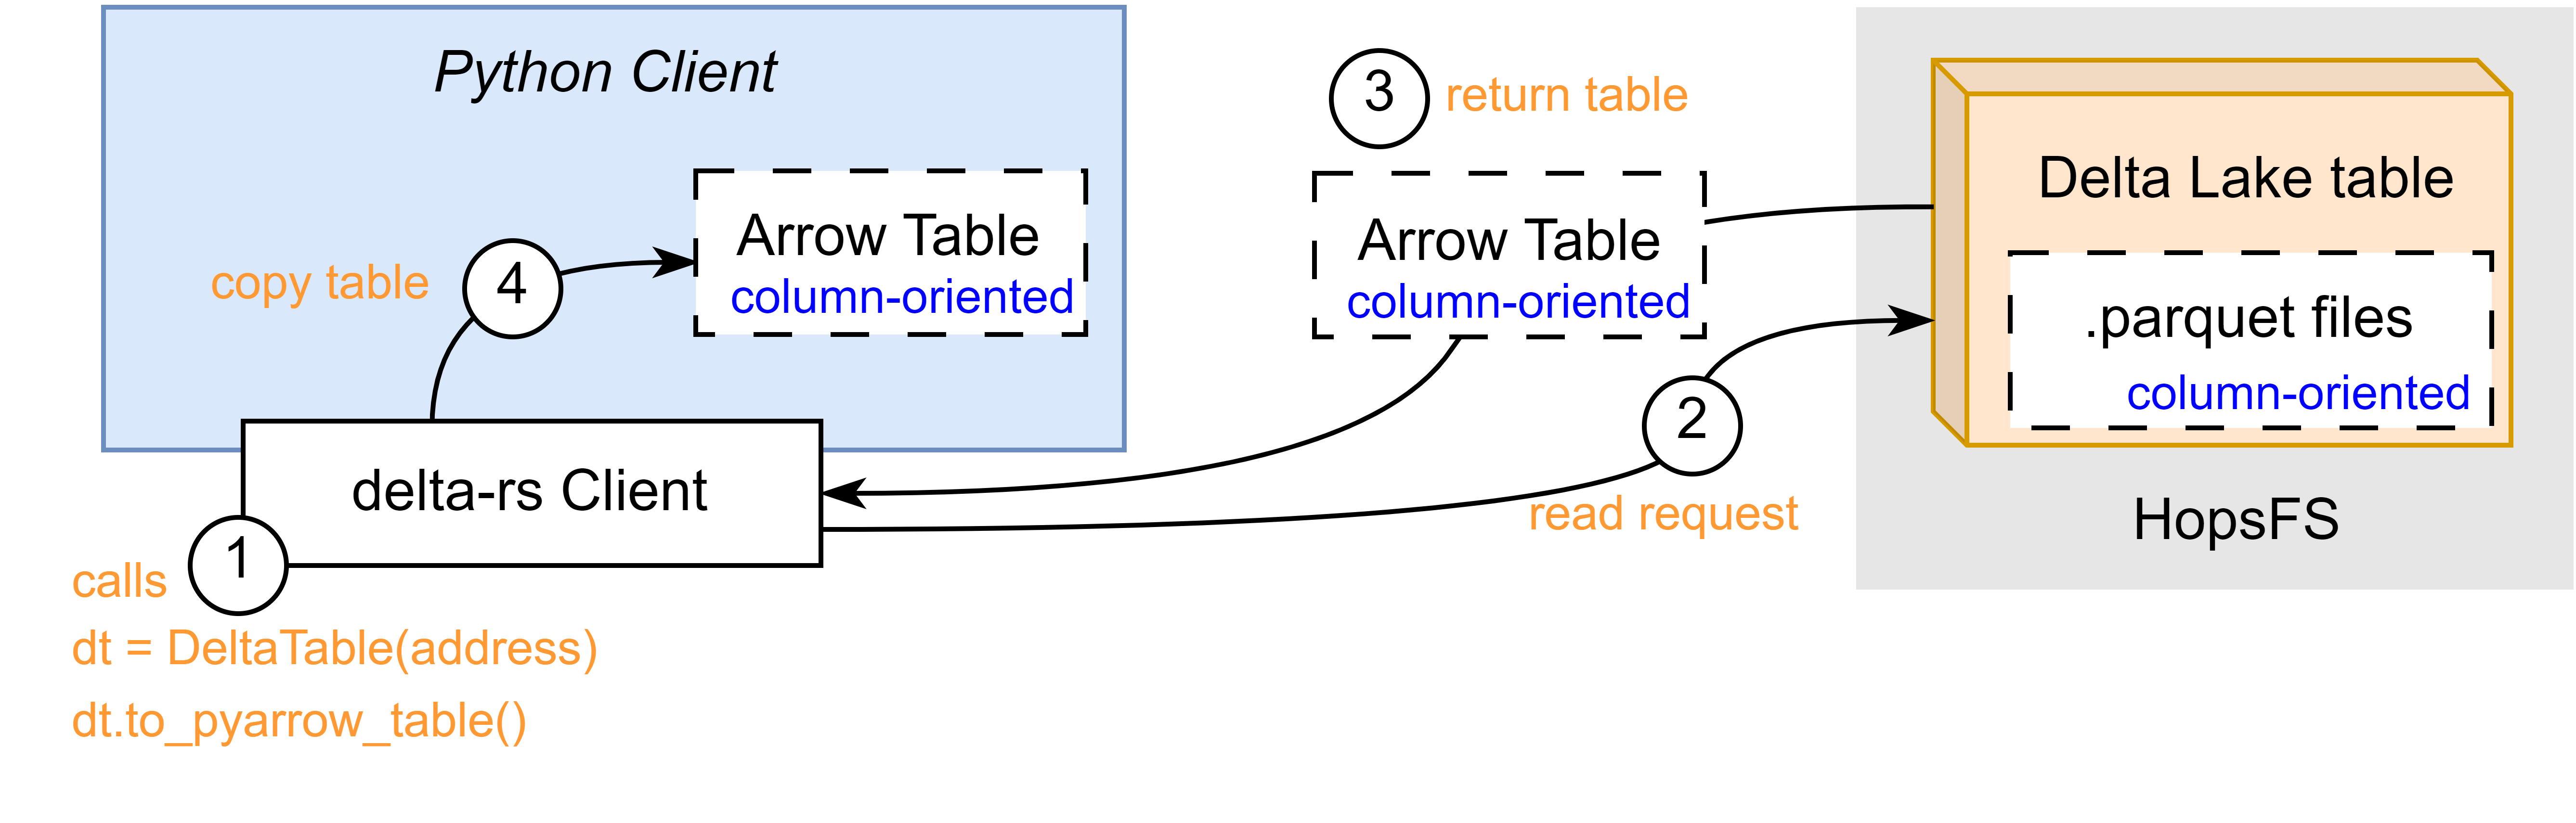
\includegraphics[width=\textwidth]{figures/2-background_and_related_work/delta_read.png}
    \end{center}
    \caption[New system - Delta Lake - read process]{Delta-rs library reading a Delta Lake table stored in \gls{HopsFS} and loading it into memory.}
    \label{fig:delta_read}
\end{figure}